\section{Название первой главы}
%Включает в себя обзор источников и раскрытие темы

Пример ссылки на Рисунок \ref{fig:choosen_words_graph} и на Таблицу \ref{tab:table1} и на Листинг \ref{lst:listing1}.


\subsection{Пример вставки и оформления рисунка}
Текст

\begin{figure}[h!]
	\centering
	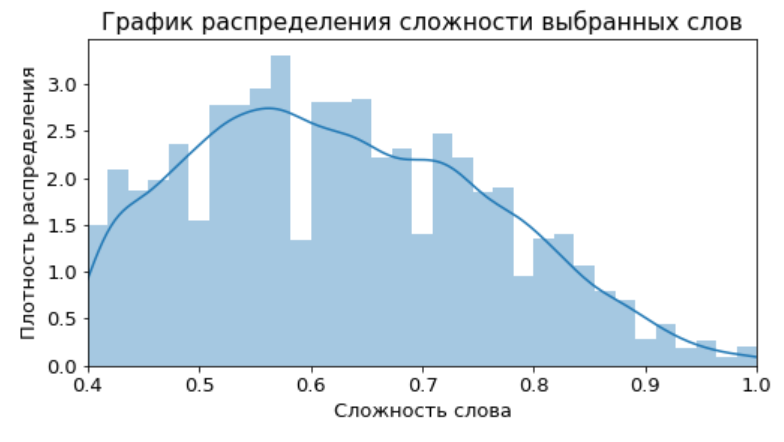
\includegraphics[scale=0.5]{images/select_sentences/choosen_words.png}
	\caption{График распределения сложности выбранных слов}
	\label{fig:choosen_words_graph}
\end{figure}

\subsection{Пример вставки и оформления кода}
Пример того как ссылаться на Листинг \ref{lst:listing1}.

\begin{lstlisting}[caption=Использование schedule в коде, label=lst:listing1]
def sched_save():
    schedule.every().hour.do(log_saver)
    while True:
        schedule.run_pending()
        time.sleep(1)
\end{lstlisting}

\subsection{Пример вставки и оформления таблицы}
Пример того как ссылаться на Таблицу \ref{tab:table1} по тексту.

\begin{table}[h!]
  \begin{center}
    \caption{Your first table.}
    \label{tab:table1}
    \begin{tabular}{l|c|r} % <-- Alignments: 1st column left, 2nd middle and 3rd right, with vertical lines in between
      \textbf{Value 1} & \textbf{Value 2} & \textbf{Value 3}\\
      $\alpha$ & $\beta$ & $\gamma$ \\
      \hline
      1 & 1110.1 & a\\
      2 & 10.1 & b\\
      3 & 23.113231 & c\\
    \end{tabular}
  \end{center}
\end{table}